\appendix
\section{NeurADP Algorithm}
\label{appendix:NeurADP}
\label{sec:alg}
\begin{algorithm}[H]
        \caption{NeurADP(N,T)}
        \begin{algorithmic}[1]
        \State Initialize: replay memory $M$, Neural value function $V$ (with random weights $\theta$)
                \For {each episode $1\leq n \leq N$}
                    \State Initialize the state $s_0^n$ by randomly positioning vehicles.
                    \State Choose a sample path $\xi^n$
                        \For {each step $0\leq t \leq T$}
                                \State Compute the feasible action set $F_t$ based on $s_t^n$.
                                \State Solve the ILP in Table 1 to get best action $a_t^n$. Add the Gaussian noise for exploration.
                                \State Store ($r_t^n,F_t$) as an experience in $M$.
                                \If {t \% updateFrequency == 0}
                                    \State Sample a random mini-batch of experiences from $M$
                                    \For {each experience $e$}
                                        \State Solve the ILP in Table 1 with the information from experience $e$ to get the objective value $y^e$
                                        \For {each vehicle $i$}
                                        \State Perform a gradient descent step on $(y^{e,i} - V(r_t^{i,n}))^2$ with respect to the network parameters $\theta$
                                        \EndFor
                                    \EndFor
                                \EndIf
                                \State Update: $s_t^{a,n}=T^a(s_t^n,a_t^n),s_{t+1}^n=T^\xi(s_t^{a,n},\xi_{t+1}^n)$
                        \EndFor
                \EndFor
        \end{algorithmic}
\end{algorithm}

% \section{Ablation study}
%\label{appendix:ablation}
%\begin{figure}[H]
%\centering
%\includegraphics[width=.45\textwidth]{Figures/50_driv_nolstm.png}
%\caption{The success rates obtained with the model for 50 drivers after removing the LSTM.}
%\label{success_rates_nolstm}
%\end{figure}

\section{Results of the original paper}
\label{appendix:original paper}

\begin{figure*}[ht!]
\centering
\captionsetup{justification=centering}
    \subcaptionbox{50 drivers}{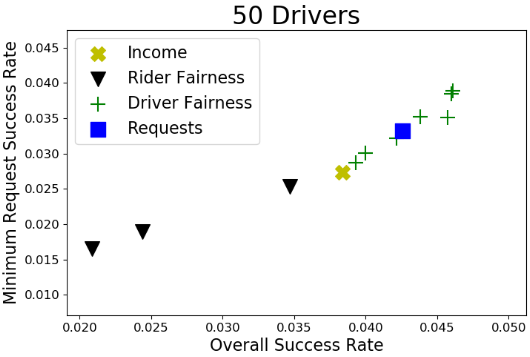
\includegraphics[width=.5\textwidth]{../openreview/Figures/50_driv_paper.png}}
    \subcaptionbox{200 drivers}{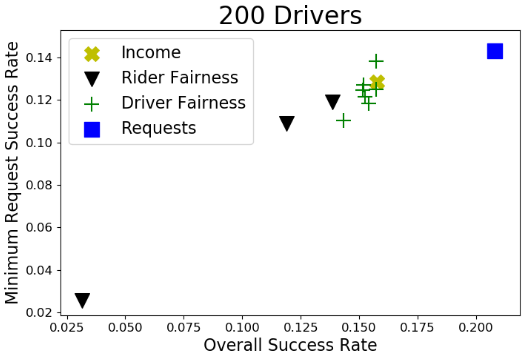
\includegraphics[width=.5\textwidth]{../openreview/Figures/200_driv_paper.png}}
    \caption{The results of the original paper \cite{raman_data-driven_2021}. The overall success rate is the rate of accepted requests in all neighborhoods, and the minimum request success rate is the minimum rate of accepted requests in a neighborhood. Each data point of the same symbol refers to a different (unspecified) value of $\lambda$.}
    \label{success_rates_paper}
\end{figure*}


\begin{figure*}[ht!]
\centering
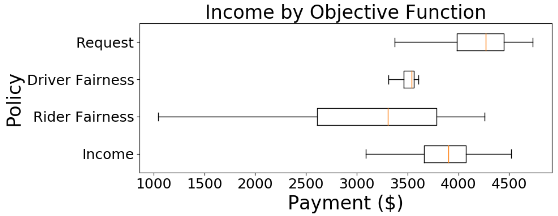
\includegraphics[width=.55\textwidth]{../openreview/Figures/200_driv_inc_paper.png}
\caption{Results of the original paper \cite{raman_data-driven_2021}. The income distribution for 200 drivers.}
\label{200_drivers_inc_paper}
\end{figure*}
